\section*{Seminár 1}

\section*{Seminár 2}

\section*{Seminár 3}

\noindent \ul{3.1} [65-D-3-N1] Pro libovolná reálná čísla $x, y$ a $z$ dokažte
nezápornost hodnoty každého z výrazů $$x^2z^2+ y^2- 2xyz, \ x^2+ 4y^2+ 3z^2- 2x
- 12y - 6z + 13, \ 2x^2+ 4y^2 + z^2- 4xy - 2xz$$ a zjistěte rovněž, kdy je
dotyčná hodnota rovna nule.

\\

\noindent \ul{3.2} [63-D-1-N1-N4]
\begin{enumerate}[a)]
\item Určete nejmenší hodnotu výrazu $V = 5 + (x - 2)^2$, $x \in \RR$. Pro která $x$ ji výraz nenabývá?

\item Určete nejmenší hodnotu výrazu $W = 9 - ab$, kde $a, b$ jsou reálná čísla splňující podmínku $a + b = 6$. Pro které hodnoty $a, b$ je $W$ minimální?

\item Určete nejmenší hodnotu výrazu $Y = 12-ab$, kde $a, b$ jsou reálná čísla splňující podmínku $a + b = 6$. Pro které hodnoty $a, b$ je $Y$ minimální?

\item Určete největší možnou hodnotu výrazu $K = 5 + ab$, kde $a, b$ jsou reálná čísla splňující podmínku $a + b = 8$. Pro které hodnoty $a, b$ je $K$ maximální?
\end{enumerate}

\\

\noindent \ul{3.3} [63-D-1] Určte, jaké nejmenší hodnoty může nabýt výraz $V
= (a-b)^2 +(b-c)^2 +(c-a)^2$, splňují-li reálná čísla $a, b, c$ dvojici podmínek
\begin{align*}
a + 3b + c &= 6,\\
-a + b - c &= 2.
\end{align*}


\\

\noindent \ul{3.4} [63-S-1] Určete, jakých hodnot může nabývat výraz $V = ab +
bc + cd + da$, splňují-li reálná čísla $a,b, c, d$ dvojici podmínek.
\begin{align*}
2a - 5b + 2c - 5d &= 4,\\
3a + 4b + 3c + 4d &= 6.
\end{align*}

\\

\noindent \ul{3.5} [65-D-3] Uvažujme výraz $$2x^2+ y^2 - 2xy + 2x + 4.$$
\begin{enumerate}[a)]

\item Najděte všechna reálná čísla $x$ a $y$, pro něž daný výraz nabývá své
nejmenší hodnoty.

\item Určete všechny dvojice celých nezáporných čísel $x$ a $y$, pro které je
hodnota daného výrazu rovna číslu 16.
\end{enumerate}

\\

\noindent \ul{3.6} [65-K-1] Najděte nejmenší možnou hodnotu výrazu $$3x^2 - 12xy
+ y^4,$$ ve kterém $x$ a $y$ jsou libovolná celá nezáporná čísla.


\\

\noindent \ul{3.7} [65-D-3-D1, resp. 61-B-S-1] . V oboru celých čísel řešte
rovnici $x^2+ y^2+ x + y = 4$.


\\

\section*{Seminár 4}

\noindent \ul{4.1} [58-S-1]
Dokažte, že pro libovolná nezáporná čísla $a, b, c$ platí $$(a + bc)(b + ac) \geq ab(c + 1)^2.$$
Zjistěte, kdy nastane rovnost.


\\

\noindent \ul{4.2} [66-D-1-N1] Dokažte, že pro libovolná reálná čísla $x$, $y$ a $z$ platí nerovnosti
\begin{enumerate}[a)]
\item $2xyz \leq x^2+ y^2z^2$,
\item $(x^2-y^2)^2\geq 4xy(x - y)^2$.
\end{enumerate}



\\

\noindent \ul{4.3} [66-D-1-N2] Dokažte, že pro libovolná kladná čísla $a$, $b$ platí nerovnost
$$\frac{a}{b^2}+ \frac{b}{a^2}\geq \frac{1}{a} + \frac{1}{b}.$$


\\

\noindent \ul{4.4} [62-D-2-N1] Dokážte nerovnosť $$\frac{1}{ab}+\frac{1}{cd}\geq \frac{8}{(a+b)(c+d)},$$ pre ľubovoľné kladné čísla $a, b, c, d$.


\\

\noindent \ul{4.5} [66-D-1] Dokažte, že pro libovolné reálné číslo $a$ platí nerovnost $$a^2+\frac{1}{a^2-a+1}\geq a+1.$$ Určte, kdy nastává rovnost.


\\

\noindent \ul{4.6} [59-D-5] Dokážte, že pre ľubovoľné kladné reálne čísla $a, b$ platí
$$ \sqrt{ab}\leq \frac{2(a^2+3ab+b^2)}{5(a+b)}\leq \frac{a+b}{2},$$
a pre každú z oboch nerovností zistite, kedy prechádza na rovnosť.


\\

\noindent \ul{4.7} [62-D-2-N1, resp. XXX FIXME]
Dokážte, že pre ľubovoľné kladné čísla $a, b, c$ platí nerovnost
$$\bigg(a +\frac{1}{b}\bigg)\bigg(b+\frac{1}{c}\bigg)\bigg(c+\frac{1}{a}\bigg)\geq 8$$
a zistite, kedy prechádza v rovnosť.


\\

\noindent \ul{4.8} [62-D-2-D2, resp. 59-K-2]
Dokážte, že pre ľubovoľné čísla $a, b$ z intervalu $\langle 1, \infty)$ platí nerovnost
$$ (a^2 + 1)(b^2 + 1) - (a - 1)^2 (b - 1)^2 \geq 4$$
a zistite, kedy nastane rovnosť.


\\

\noindent \ul{4.9} [58-D-6]
Dokažte, že pro libovolná různá kladná čísla $a, b$ platí
$$\frac{a+b}{2}<\frac{2(a^2 + ab + b^2 )}{3(a+b)}<\sqrt{\frac{a^2+b^2}{2}}.$$


\\

\section*{Seminár 5}

\noindent \ul{5.1} [60-D-1-N1] Máme tri čísla so súčtom 2010, pričom každé z nich je aritmetickým priemerom zvyšných dvoch. Aké sú to čísla?


\\

\noindent \ul{5.2} [60-D-1-N2] Máme tři čísla, o nichž víme, že každé z nich je aritmetickým
průměrem některých dvou z našich tří čeísel. Dokažte, že naše tři čísla jsou stejná.


\\

\noindent \ul{5.3} [60-D-1]
Lucia napísala na tabuľu dve nenulové čísla. Potom medzi ne postupne vkladala znamienka plus, mínus, krát a delené a všechny štyri príklady správne vypočítala. Medzi výsledkami boli iba dve rôzne hodnoty. Aké dve čísla mohla Lucia na tabuľu napísať?


\\

\noindent \ul{5.4} [60-K-1]
Na tabuli sú napísané práve tri (nie nutne rôzne) reálne čísla. Vieme, že súčet ľubovoľných dvoch z nich je tam napísaný tiež. Určte všechny trojice takých čísel.


\\

\noindent \ul{5.5} [60-S-1]
Po okruhu behajú dvaja atléti, každý inou konštantnou rýchlosťou. Keď bežia opačnými smermi, stretávajú sa každých 10 minút, keď bežia rovnakým smerom, stretávajú sa každých 40 minút. Za aký čas zabehne okruh rýchlejší atlét?


\\

\noindent \ul{5.6} [66-D-4-N1] Určete všechny dvojčleny $P (x) = ax + b$, pro které platí $P(2) = 3$
a $P (3) = 2$.


\\

\noindent \ul{5.7} [66-D-4-N2] Určete všechny trojčleny $P (x) = ax^2+ bx + c$, pro které platí $P
(1) = 4$, $P (2) = 9$ a $P (3) = 18$.


\\

\noindent \ul{5.8} [66-D-4-N3] Určete všechny dvojčleny $P (x) = ax+b$ s celočíselnými koeficienty
$a$ a $b$, pro které platí $P (1) < P (2)$ a $P (1)^2+ P(2)^2= 5$.


\\

\noindent \ul{5.9} [66-D-4-D2] Koeficienty $a, b, c$ trojčlenu $P (x) = ax^2+ bx + c$ jsou reálná
čísla, přitom každá ze tří jeho hodnot $P (1), P (2)$ a $P (3)$ je celým číslem. Plyne odtud, že
také čísla $a, b, c$ jsou celá, nebo je nutně celé aspoň některé z nich (které)?


\\

\noindent \ul{5.10} [59-S-3] Nájdite všechny dvojice nezáporných celých čísel $a$, $b$, pro které platí
$$a^2 + b + 2 = a + b^2.$$


\\

\noindent \ul{5.11} [66-D-4]
Najděte všechny trojčleny $P(x)=ax^2+bx+c$ s celočíselnými koeficienty $a, b, c$, pro které platí $P(1) < P(2) < P(3)$ a zároveň $$(P(1))^2+ (P(2))^2+ (P(3))^2= 22.$$

\\

\noindent \ul{5.12} [62-K-3]
Nájdite všechny dvojice celých kladných čísel $a$ a $b$, pre ktoré je číslo $a^2 +b$ o~62 väčšie
ako číslo $b^2 + a$.


\\

\noindent \ul{5.13} [60-D-1-D1] Nech $n$ je prirodzené číslo väčšie ako 2. Máme $n$ čísel so súčtom $n$, pričom každé z nich je aritmetickým priemerom ostatných čísel. Aké sú to čísla?


\\

\section*{Seminár 6}

\noindent \ul{6.1} [Holton, 4.2, problem 38, str. 115] Nech $N$ je päťciferné kladné číslo také, že $N=\overline{a679b}$. Ak je $N$ deliteľné 72, určte prvú cifru $a$ a poslednú cifru $b$.


\\

\noindent \ul{6.2} [66-D-2-N1] Dokažte, že v nekonečné řadě čísel
$$ 1 \cdot 2 \cdot 3, 2 \cdot 3 \cdot 4, 3 \cdot 4 \cdot 5, 4 \cdot 5 \cdot 6, \ldots ,$$
je číslo první dělitelem všech čísel dalších.


\\

\noindent \ul{6.3} [63-D-5-N1] Dokažte, že pro každé přirozené číslo $n$ je číslo
$n^3+ 2n$ dělitelné třemi.


\\

\noindent \ul{6.4} [63-D-5-N2] Dokažte, že pro každé liché číslo $n$ je číslo
$n^2 - 1$ dělitelné osmi.


\\

\noindent \ul{6.5} [63-D-5-N3+63-D-5-N4, resp. C-55-I-1] \begin{enumerate}[a)]
\item Dokažte, že pro všechna kladná celá čísla $m$ je rozdíl $m^6 - m^2$ dělitelný šedesáti.
\item Určte všechna kladná celá čísla $m$, pro která je rozdíl $m^6 - m^2$ dělitelný číslem 120.
\end{enumerate}

\\

\noindent \ul{6.6} [59-K-1]
Dokážte, že pre ľubovoľné celé čísla $n$ a $k$ väčšie ako 1 je číslo $n^{k+2} - n^k$ deliteľné dvanástimi.


\\

\noindent \ul{6.7} [58-S-3] Jestliže jistá dvě přirozená čísla ve stejném pořadí sečteme, odečteme,
vydělíme a vynásobíme a všechny čtyři vysledky sečteme, dostaneme 2009. Určete tato dvě čísla.

\\

\noindent \ul{6.8} [66-D-2-N2] Najděte všechna celá $d > 1$, při nichž hodnoty výrazů $U(n) = n^3+
17n^2-1$ a $V (n) = n^3+ 4n^2+ 12$ dávají při dělení číslem $d$ stejné zbytky, ať je celé číslo
$n$ zvoleno jakkoli.


\\

\noindent \ul{6.9} [66-D-2-D1] Pro která přirozená čísla $n$ není výraz $V (n) = n^4+ 11n^2 - 12$ násobkem osmi?


\\

\noindent \ul{6.10} [66-D-2]
Najděte největší přirozené číslo $d$, které má tu vlastnost, že pro libovolné přirozené $n$ je hodnota výrazu $$V (n) = n^4+ 11n^2-12$$
dělitelná číslem $d$.


\\

\noindent \ul{6.11} [66-S-2]
Označme $M$ množinu všetkých hodnôt výrazu $V (n) = n^4 + 11n^2 - 12$, pričom $n$ je nepárne prirodzené číslo. Nájdite všechny možné zvyšky po delení číslom 48, ktoré dávajú prvky množiny $M$.


\\

\noindent \ul{6.12} [60-D-2]
Dokážte, že výrazy $23x + y$, $19x + 3y$ sú deliteľné číslom 50 pre rovnaké dvojice prirodzených čísel $x$, $y$.


\\

\section*{Seminár 7}

\noindent \ul{7.1} [61-D-3-N1] Určte, pre ktoré prirodzené čísla $a, b$ platí $(a, b) = 10$ a zároveň  $[a, b] = 150$.


\\

\noindent \ul{7.2} [69-D-5-N1] Nech $d$ je najväčší spoločný deliteľ prirodzených čísel $a$ a $b$. Ukážte, že čísla $a/d$ a $b/d$ sú celé a nesúdeliteľné.


\\

\noindent \ul{7.3} [60-D-5-N2] Dokážte, že pre ľubovoľné prirodzené čísla $a, b$ platí vzťah $[a, b] \cdot (a, b) = ab$.


\\

\noindent \ul{7.4} [64-D-5-N4] Platí pre každé tri prirodzené čísla $a, b, c$ a ich najväčší spoločný deliteľ $d$ a ich najmenší spoločný násobok $n$ rovnosť $abc = nd$?


\\

\noindent \ul{7.5} [64-D-5-N5] Ak majú prirodzené čísla $a, b$ najväčšieho spoločného deliteľa $d$, majú rovnakého najväčšieho spoločného deliteľa aj čísla $a$, $b$, $a - b$, $a + b$. Dokážte. Platí rovnaké tvrdenie pre najmenší spoločný násobok?


\\

\noindent \ul{7.6} [61-D-3-N4, resp. 50-C-II-1] Nájdite všechny dvojice prirodzených čísel $a, b$, pro které platí $a+b+[a, b]+(a, b) = 50$.


\\

\noindent \ul{7.7} [61-S-1]
Nájdite všechny dvojice prirodzených čísel $a, b$, pro které platí rovnosť množín
$$\{a \cdot [a, b], b \cdot (a, b)\} = \{45, 180\}.$$


\\

\noindent \ul{7.8} [64-D-5]
Rozdiel dvoch prirodzených čísel je $2010$ a ich najväčší spoločný deliteľ je $2014$-krát menší ako ich najmenší spoločný násobok. Určte všechny také dvojice čísel.


\\

\noindent \ul{7.9} [60-D-5-D3] Nájdite všechny dvojice kladných celých čísel $a, b$, pre ktoré má výraz
$$\frac{a}{b}+\frac{14b}{9a}$$
celočíselnú hodnotu.


\\

\noindent \ul{7.10} [60-D-5]
Dokážte, že najmenší spoločný násobok $[a, b]$ a najväčší spoločný deliteľ $(a, b)$ ľubovoľných dvoch kladných celých čísel $a, b$ spĺňajú nerovnosť
$$a \cdot (a, b) + b \cdot [a, b] \geq 2ab.$$
Zistite, kedy v tejto nerovnosti nastane rovnosť.


\\

\noindent \ul{7.11} [61-D-3]
Nájdite všechny trojice prirodzených čísel $a, b, c$, pro které platí množinová rovnosť
$$\{(a, b), (a, c), (b, c), [a, b], [a, c], [b, c]\}= \{2, 3, 5, 60, 90, 180\},$$
pričom $(x, y)$ a $[x, y]$ označuje postupne najväčší spoločný deliteľ a najmenší spoločný násobok čísel $x$ a $y$.


\\

\noindent \ul{7.12} [63-S-2] Čísla 1, 2, \ldots , 10 rozdělte do dvou skupin
tak, aby nejmenší společný násobek součinu všech čísel první skupiny a součinu
všech čísel druhé skupiny byl co nejmenší. Stačí, když uvedete jedno rozdělení a
zdůvodníte, proč má požadovanou vlastnost.


\\

\section*{Seminár 8}

\noindent \ul{8.1} [59-D-6-N1, Sedláček, J.: Co víme o přirozených číslech, str. 7] Trojciferné číslo sa končí cifrou 4. Ak túto cifru presunieme na prvé miesto (a ostatné dve cifry necháme bez zmeny), dostaneme číslo, ktoré je o 81 menšie ako pôvodné číslo. Určte pôvodné číslo.


\\

\noindent \ul{8.2} [Holton, 4.1 -- problem 20, str. 110] Nájdite všechny prirodzené dvojciferné čísla, ktoré sa rovnajú dvojnásobku súčinu svojich cifier.


\\

\noindent \ul{8.4} [61-K-2] Janko má tri kartičky, na každej je iná nenulová cifra. Súčet všetkých trojciferných čísel, ktoré možno z týchto kartičiek zostaviť, je číslo o 6 väčšie ako trojnásobok jedného z nich. Aké cifry sú na kartičkách?


\\

\noindent \ul{8.5} [63-K-1]
Nájdite všechny trojice (nie nutne rôznych) cifier $a, b, c$ také, že päťciferné čísla $\overline{6abc3}$ a $\overline{3abc6}$ sú v pomere 63 : 36.


\\

\noindent \ul{8.6} [57-D-6-D2 resp. 53-C-II-4]  Žáci měli vypočítat příklad $x + y \cdot z$ pro
trojciferné číslo $x$ a dvojciferné číslo $y, z$. Martin umí násobit a sčítat čísla zapsaná v
desítkové soustavě, al ezapomněl na prvido přednosti násobení před sčítáním. Proto mu vyšlo sice
zajímavé číslo, které se čte stejně zleva doprava jako zprava doleva, správný výsledek byl ale o
2004 menší. Určete čísla $x, y, z$.


\\

\noindent \ul{8.7} [58-D-3-N1 resp. 56-C-S-1] Určete počet všech čtyřmístných přirozených čísel,
která jsou delitená šesti a v jejichž zapisu se vyskytují právě dvě jedničky.

\\

\noindent \ul{8.8} [58-D-3-N2 resp.54-C-I-5]  Uečete počet všech trojic dvojmístných přirozených
čísel $a$, $b$, $c$, jejichž součin $abc$ má zápis, ve kterém jsou všechny číslice stejné. Trojice
lišící se pouze pořadím čísel považujeme za stejné, tj. započítáváme je pouze jednou.


\\

\noindent \ul{8.9} [58-D-3] Najděte všechny čtyřmístná čísla $n$, která mají následující tři
vlastnosti: V zápise čísla $n$ jsou dvě různé číslice, každá dvakrát. Číslo $n$ je dělitelné sedmi.
Číslo, které vznikne obrácením pořadí číslic čísla $n$, je rovněž čtyřmístné a dělitelné sedmi.


\\

\noindent \ul{8.10} [57-D-6] Klárka měla na papíru napsáno trojmístné číslo. Když ho správně
vynásobila devíti, dostala čtyřmístné číslo, jež začínalo touž číslicí jako číslo původní,
prostřední dvě číslice se rovnaly a poslední číslice byla součtem číslic původního čísla. Které
čtyřmístné číslo mohla Klárka dostat?


\\

\section*{Seminár 9}

\noindent \ul{9.1} Dokážte, že súčet veľkostí vnútorných uhlov ľubovoľného trojuholníka je $180^\circ$.


\\

\noindent \ul{9.2} [66-D-3-N1] Z trojuholníkových nerovností medzi dĺžkami strán ľubovoľného trojuholníka odvoďte známe
pravidlo $\alpha < \beta \Rightarrow a < b$ o porovnaní veľkostí vnútorných uhlov a dĺžok protiľahlých strán v ľubovoľnom trojuholníku $ABC$.


\\

\noindent \ul{9.3} [63-D-4-N3] Dokažte věty:

a) Mají-li dva trojúhelníky stejnou výšku, pak poměr jejich obsahů se rovná poměru délek příslušných základen.

b) Mají-li dva trojúhelníky shodné základny, pak poměr jejich obsahů se rovná poměru příslušných výšek.


\\

\noindent \ul{9.4} [61-D-5-N1]  Pre všeobecný trojuholník $ABC$ so stranami $a$, $b$, $c$ a obsahom $S$ platí pre polomer $r$ vpísanej kružnice vzorec $r = 2S/(a + b + c)$. Dokážte.


\\

\noindent \ul{9.5} Dokážte, že uhlopriečky v rovnobežníku sa navzájom polia.


\\

\noindent \ul{9.6} [58-D-4-N1]  Označme $U$ průsečík úhlopříček daného konvexního čtyřúhelníku
$ABCD$. Dokážte, že přímky $AB$ a $CD$ jsou rovnoběžné, právě když trojúhelníky $ADP$ a $BCP$
mají stejný obsah.

\\

\noindent \ul{9.7} [64-D-4-N1] Lichobežník $ABCD$ má základne s dĺžkami $|AB|=a$ a $|CD|=C$ a jeho uhlopriečky sa pretínajú v bode $U$. Aký je pomer obsahov trojuholníkov $ABU$ a $CDU$?


\\

\noindent \ul{9.8} [58-D-2-D1] Nechť $k$ je kružnice opsaná pravúhlému trojúhelníku $ABC$ s
přeponou $AB$ délky $c$. Označme $S$ střed strany $AB$ a $D$ a $E$ průsečíky os stran $BC$ a $AC$
s týmž obloukem $AB$ kružnice $k$. Vyjádřete obsah trojúhelníku $DSE$ pomocí délky přepony $c$.


\\

\noindent \ul{9.9} [58-D-2-D2] Vyjádřete obsah rovnoramenného lichoběžníku $ABCD$ se základnami $AB$
a $CD$ pomocí délek $a$, $c$ jeho základny a délky $b$ jeho ramen.


\\

\noindent \ul{9.10} Použitím viet o podobnosti trojuholníkov a Pytagorovej vety odvoďte Euklidove vety o odvesne a o výške pravouhlého trojuholníka.

\\

\section*{Seminár 10}

\noindent \ul{10.1} [66-S-3] Päta $P$ výšky z vrcholu $C$ v trojuholníku $ABC$ delí stranu $AB$ v pomere $|AP| : |PB|= 1 : 3$. V rovnakom pomere sú aj obsahy štvorcov nad jeho stranami $AC$ a $BC$.
Dokážte, že trojuholník $ABC$ je pravouhlý.

\\

\noindent \ul{10.2} [66-D-3]
Päta výšky z vrcholu $C$ v trojuholníku $ABC$ delí stranu $AB$ v pomere $1 : 2$. Dokážte, že pri zvyčajnom označení dĺžok strán trojuholníka $ABC$ platí nerovnost $$3|a - b| < c.$$

\\

\noindent \ul{10.3} [63-S-3] Je dán trojúhelník $ABC$ s pravým úhlem při vrcholu
$C$. Středem $I$ kružnice trojúhelníku vepsané vedeme rovnoběžky se stranami
$CA$ a $CB$, které protnou přeponu postupně v bodech $X$ a $Y$. Dokažte, že
platí $|AX|^2 + |BY |^2 = |XY |^2$.


\\

\noindent \ul{10.4} [58-S-2] V pravoúhlém trojúhelníku $ABC$ označíme $P$ patu výšky z vrcholu $C$
 na přeponu $AB$. Průsečík úsečky $AB$ s přímkou, která prochází vrcholem $C$ a středem kružnice
 vepsané trojúhelníku $PBC$, označíme $D$. Dokažte, že úsečky $AD$ a $AC$ jsou shodné.


\\

\noindent \ul{10.5} [64-D-4] Označme $E$ stred základne $AB$ lichobežníka $ABCD$, v ktorom platí $|AB| : |CD| = 3 : 1$. Uhlopriečka $AC$ pretína úsečky $ED$, $BD$ postupne v bodoch $F$, $G$. Určte postupný pomer $|AF| : |FG| : |GC|$.


\\

\noindent \ul{10.6} [63-D-4] Ve čtverci $ABCD$ označme $K$ střed strany $AB$ a
$L$ střed strany $AD$. Úsečky $KD$ a $LC$ se protínají v bodě $M$ a rozdělují
čtverec na dva trojúhelníky a dva čtyřúhelníky. Vypočtetě jejich obsahy,
jestliže úsečka $LM$ má délku 1\,cm.

\\

\noindent \ul{10.7} [65-K-3] V pravoúhlém lichoběžníku $ABCD$ s pravým vrcholem
u vrcholu $A$ základny $AB$ je bod $K$ průsečíkem výšky $CP$ lichoběžníku s
jeho úhlopříčkou $BD$. Obsah čtyřúhelníku $APCD$ je polovinou obsahu
lichobežníku $ABCD$. Určete, jakou část obsahu trojúhelníku $ABC$ zaujímá
trojúhelník $BCK$.


\\

\noindent \ul{10.8} [58-D-2] Pravouhlému trojuholníku $ABC$ s preponou $AB$ je opísaná kružnica. Päty kolmíc z bodov $A$, $B$ na dotyčnicu k tejto kružnici v bode $C$ označme $D$, $E$. Vyjadrite dĺžku úsečky $DE$ pomocou dĺžok odvesien trojuholníka $ABC$.


\\

\noindent \ul{10.9} [58-K-2]
V pravouhlom trojuholníku $ABC$ označíme $P$ pätu výšky z vrcholu $C$ na preponu $AB$ a $D, E$ stredy kružníc vpísaných postupne trojuholníkom $APC$, $CPB$. Dokážte, že stred
kružnice vpísanej trojuholníku $ABC$ je priesečníkom výšok trojuholníka $CDE$.


\\

\section*{Seminár 11}

\noindent \ul{11.1} [57-S-2] V daném rovnobežníku $ABCD$ je bod $E$ střed strany $BC$ a bod $F$ leží
uvnitř strany $AB$. Obsah trojúhelníku $AFD$ je $15$\,cm$^2$ a obsah trojúhelníku $FBE$ je
$14$\,cm$^2$. Určte obsah čtyřúhelníku $FECD$.


\\

\noindent \ul{11.2} [62-K-2] Vnútri rovnobežníka $ABCD$ je daný bod $K$ a v páse medzi rovnobežkami $BC$ a $AD$ v polrovine opačnej k $CDA$ je daný bod $L$. Obsahy trojuholníkov $ABK, BCK, DAK$ a $DCL$ sú $S_{ABK} = 18$\,cm$^2$, $S_{BCK} = 8$\,cm$^2$, $S_{DAK} = 16$\,cm$^2$, $S_{DCL} = 36$\,cm$^2$. Vypočítajte obsahy trojuholníkov $CDK$ a $ABL$.


\\

\noindent \ul{11.3} [64-S-2] Označme $K$ a $L$ postupne body strán $BC$ a $AC$ trojuholníka $ABC$, pro které platí $|BK|= \frac{1}{3}|BC|$, $|AL| =\frac{1}{3}|AC|$. Nech $M$ je priesečník úsečiek $AK$ a $BL$. Vypočítajte pomer obsahov trojuholníkov $ABM$ a $ABC$.


\\

\noindent \ul{11.4} [64-K-3]  Daný je lichobežník $ABCD$ so základňami $AB$, $CD$, pričom $2|AB| = 3|CD|$.

a) Nájdite bod $P$ vnútri lichobežníka tak, aby obsahy trojuholníkov $ABP$ a $CDP$ boli v pomere $3 : 1$ a aj obsahy trojuholníkov $BCP$ a $DAP$ boli v pomere $3 : 1$.

b) Pre nájdený bod $P$ určte postupný pomer obsahov trojuholníkov $ABP$, $BCP$, $CDP$ a $DAP$.


\\

\noindent \ul{11.5} [62-D-6] Vnútri pravidelného šesťuholníka $ABCDEF$ s obsahom 30\,cm$^2$ je zvolený bod $M$. Obsahy trojuholníkov $ABM$ a $BCM$ sú postupne 3\,cm$^2$ a 2\,cm$^2$. Určte obsahy trojuholníkov $CDM$, $DEM$, $EFM$ a $FAM$.


\\

\noindent \ul{11.6} [65-D-4] Uvnitř stran $AB$, $AC$ daného trojuholníku $ABC$
jsou zvoleny po řadě body $E$, $F$, přičemž $EF \parallel BC$. Úsečka $EF$ je
pak rozdělena bodem $D$ tak, že platí $$p = |ED| : |DF | = |BE| : |EA|.$$

a) Ukažte, že poměr obsahů trojúhelníků $ABC$ a $ABD$ je pro $p = 2 : 3$ stejný jako pro $p = 3 : 2$.

b) Zdůvodněte, proč poměr obsahů trojúhelníků $ABC$ a $ABD$ má hodnotu nejméně 4.


\\

\section*{Seminár 12}

\noindent \ul{12.1} [57-K-1] Trojúhelník $ABC$ splňuje při obyvyklém značení délek stran podmínku $a
\leq b \leq c$. Vepsaná kružnice se dotýká stran $AB$, $BC$ a $AC$ postupně v bodech $K$, $L$ a $M$.
Dokažte, že z úseček $AK$, $BL$ a $CM$ lze sestroj trojúhelník, právě když platí $b + c <
3a$.


\\

\noindent \ul{12.2} [61-S-2] Označme $S$ stred základne $AB$ daného rovnoramenného trojuholníka $ABC$. Predpokladajme, že kružnice vpísané trojuholníkom $ACS$, $BCS$ sa dotýkajú priamky $AB$ v~bodoch, ktoré delia základňu $AB$ na tri zhodné diely. Vypočítajte pomer $|AB| : |CS|$.


\\

\noindent \ul{12.3} [62-S-1] Danému rovnostrannému trojuholníku vpíšme a opíšme kružnicu. Označme $S$ obsah vzniknutého medzikružia a $T$ obsah kruhu, ktorého priemer je zhodný s dĺžkou strany daného trojuholníka. Ktorý z obsahov $S$, $T$ je väčší? Svoju odpoveď zdôvodnite.


\\

\noindent \ul{12.4} [61-D-5] Daný je rovnoramenný trojuholník so základňou dĺžky $a$ a ramenami dĺžky $b$. Pomocou nich vyjadrite polomer $R$ kružnice opísanej a polomer $r$ kružnice vpísanej tomuto trojuholníku. Potom ukážte, že platí $R \geq 2r$ a zistite, kedy nastane rovnosť.


\\

\noindent \ul{12.5} [63-D-2]  V rovině jsou dány body $A$, $P$, $T$ neležící na
přímce. Sestrojte trojúhelník $ABC$ tak, aby $P$ byla pata jeho výšky z vrcholu
$A$ a $T$ bod dotyku strany $AB$ s kružnicí mu vepsanou. Proveďte diskusi počtu
řešení vzhledem k poloze daných bodů.

\\

\noindent \ul{12.6} [59-D-4] Kružnica $k(S; r)$ sa dotýka priamky $AB$ v bode $A$. Kružnica $l(T; s)$ sa dotýka priamky $AB$ v bode $B$ a pretína kružnicu k v krajných bodoch $C$, $D$ jej priemeru. Vyjadrite dĺžku a úsečky $AB$ pomocou polomerov $r$, $s$. Dokážte ďalej, že priesečník $M$ priamok $CD$, $AB$ je stredom úsečky $AB$.


\\

\noindent \ul{12.7} [61-D-2] Dĺžky strán trojuholníka sú v metroch vyjadrené celými číslami. Určte ich, ak má trojuholník obvod 72\,m a ak je najdlhšia strana trojuholníka rozdelená bodom dotyku vpísanej kružnice v pomere $3 : 4.$


\\

\section*{Seminár 13}

\section*{Seminár 14}

\section*{Seminár 15}

\section*{Seminár 16}

\section*{Seminár 17}

\section*{Seminár 18}

\noindent \ul{18.1} [59-S-1]
 Ak zväčšíme čitateľ aj menovateľ istého zlomku o 1, dostaneme zlomok o~hodnotu 1/20 väčší. Ak urobíme s väčším zlomkom rovnakú operáciu, dostaneme zlomok o~hodnotu 1/12 väčší, ako bola hodnota zlomku na začiatku. Určte všechny tri zlomky.


\\

\noindent \ul{18.2} [59-D-3-N1] Určte $\lfloor 0 \rfloor, \lfloor 3{,}5 \rfloor,\lfloor 2{,}1\rfloor, \lfloor -4 \rfloor, \lfloor -3{,}9 \rfloor, \lfloor -0{,}2\rfloor$. Symbol $\lfloor x\rfloor$ označuje najväčšie celé číslo, ktoré nie je väčšie ako číslo $x$, tzv. dolnú celú časť reálneho čísla $x$.


\\

\noindent \ul{18.3} [59-D-3-N2] Nech $a$ je celé číslo a $t \in \langle 0; 1)$. Určte $\lfloor a \rfloor, \lfloor a+t \rfloor,\lfloor a+\frac{1}{2}t\rfloor, \lfloor a-t \rfloor, \\ \lfloor a+2t \rfloor, \lfloor a-2t\rfloor$.


\\

\noindent \ul{18.4} [59-D-3]
Určte všechny reálne čísla $x$, ktoré vyhovujú rovnici $4x - 2\lfloor x\rfloor = 5$.


\\

\noindent \ul{18.5} [57-D-3-N1] Určete všechna celá čísla $n$, pro která nabývá zlomek $(4n + 27)/(n + 3)$ celočíselné
hodnoty.


\\

\noindent \ul{18.6} [57-D-3] Máme určitý počet krabiček a určitý počet kuliček. Dáme-li do každé
krabičky právě jednu kuličku, zůstane nám $n$ kuliček. Když však necháme právě $n$ krabiček stranou,
můžeme všechny kuličky rozmístit tak, aby jich v každé zbývající krabičce bylo právě $n$. Kolik máme
krabiček a kolik kuliček?


\\

\noindent \ul{18.7} [57-K-4]
Najděte všechny trojice celých čísel $x, y, z$, pro které platí
$$x+y\sqrt{3}+z\sqrt{7}=y+z\sqrt{3}+x\sqrt{7}. $$

\\

\noindent \ul{18.8} [64-D-1]
Určte všechny dvojice $(x, y)$ reálnych čísel, ktoré vyhovujú sústave rovníc
\begin{align*}
\sqrt{(x + 4)^2} &= 4 - y,\\
\sqrt{(y - 4)^2} &= x + 8.
\end{align*}


\\

\noindent \ul{18.9} [59-K-4] Určte všechny dvojice reálnych čísel $x, y$, ktoré vyhovujú sústave rovníc
\begin{align*}
\lfloor x + y\rfloor &= 2 010,\\
\lfloor x\rfloor - y &= p,
\end{align*}
ak a) $p = 2$, b) $p = 3$.
Symbol $\lfloor x \rfloor$ označuje najväčšie celé číslo, ktoré nie je väčšie ako dané reálne číslo $x$ (tzv. dolná celá časť reálneho čísla $x$).


\\

\noindent \ul{18.10} [64-S-1]
V obore reálnych čísel vyriešte sústavu rovníc
\begin{align*}
|1 - x| &= y + 1,\\
|1 + y| &= z - 2,\\
|2 - z| &= x - x^2.
\end{align*}

\\

\section*{Seminár 19}

\noindent \ul{19.1} [63-D-3-N2] Číslo $n$ je součinem dvou různých prvočísel.
Zvětšíme-li menší z nich o 1 a druhé ponecháme, jejich součin se zvětší o 7.
Určete číslo $n$.

\\

\noindent \ul{19.2} [63-D-3-N4] Číslo $n$ je součinem dvou prvočísel.
Zvětšíme-li každé z nich o 1, jejich součen se zvětší o 35. Určete číslo $n$.

\\

\noindent \ul{19.3} [63-D-3] Číslo $n$ je součinem dvou prvočísel. Zvětšíme-li
každé z nich o 1 a druhé o 1 zmenšíme, jejich součin zůstane stejný. Určete
číslo n $n$.

\\

\noindent \ul{19.4} [64-S-3]
Nájdite najmenšie prirodzené číslo $n$ s ciferným súčtom 8, ktoré sa rovná súčinu troch rôznych prvočísel, pričom rozdiel dvoch najmenších z nich je 8.


\\

\noindent \ul{19.5} [57-S-1]
Najděte všechny dvojice přirozených čísel $a, b$ větších než 1 tak, aby jejich součet i součin byly mocniny prvočísel.


\\

\noindent \ul{19.6} [65-D-1-D2 resp. 55-C-II-4] Najděte všechny dvojice
prvočísel $p$ a $q$, pro které platí $p + q^2= q + 145p^2$.


\\

\noindent \ul{19.7} [66-D-2-D4, resp. 62-D-5]
Určte všechny celé čísla $n$, pre ktoré $2n^3 -3n^2 +n+3$ je prvočíslo.


\\

\noindent \ul{19.8} [MŘMUI, 2.3, str 174] Nájdite všechny prvočísla, ktoré sú súčasne súčtom a rozdielom dvoch vhodných prvočísel.


\\

\noindent \ul{19.9} [Thiele, str. 95] Nájdite celočíselné riešenia rovnice $$\frac{1}{x}+\frac{1}{y}=\frac{1}{p},$$ kde $p$ je pevne dané prvočíslo.


\\

\noindent \ul{19.10} [65-D-1]
Najděte všechny možné hodnoty součinu prvočísel $p$, $q$, $r$, pro které platí
$$p^2 - (q + r)^2= 637.$$


\\

\section*{Seminár 20}

\noindent \ul{20.1} [65-K-4] Adam s Bárou hrají se zlomkem
$$ \frac{10a + b}{10c + d}$$ takovou hru na čtyří tahy: Hráči střídavě nahrazují libovolné z dosud
neurčených písmen $a$, $b$, $c$, $d$ nějakou číslicí 1 do 9. Bára vyhraje, když výsledný zlomek bude
roven buď celému číslu, nebo číslu s konečným počtem desetinných míst; jinak vyhraje Adam (například
když vznikne zlomek $\frac{11}{29}$). Začíná-li Adam, jak má hrát Bára, aby zaručeně vyhrála?
Začíná-li Bára, je možné poradit Adamovi tak, aby vždy vyhrál?


\\

\noindent \ul{20.2} [57-D-1-N1] Jsou-li $m, k$ a $\sqrt[k]{m}$ celá čísla větší než 1, pak v
rozkladu čísla $m$ na prvočinitele se každé prvočíslo vyskytuje vmocnině, jejíž mocnitel je násobkem
čísla $k$. Dokažte.


\\

\noindent \ul{20.3} [57-D-1]
Určete nejmenší přirozené číslo $n$, pro než i čísla
$\sqrt{2n}, \sqrt[3]{3n}, \sqrt[5]{5n}$ jsou přirozená.


\\

\noindent \ul{20.4} [60-K-2]
Nájdite všechny kladné celé čísla $n$, pre ktoré je číslo $n^2 + 6n$ druhou mocninou celého čísla.


\\

\noindent \ul{20.5} [66-K-1] Nájdite všechny mnohočleny $P(x) = ax^2 +bx+c$ s celočíselnými koeficientami spĺňajúce
$$1 < P(1) < P(2) < P(3) \ \ \ \text{a súčasne} \ \  \
\frac{P(1) \cdot P(2) \cdot P(3)}{4}= 17^2.$$


\\

\noindent \ul{20.6} [64-K-1]
Celé čísla od 1 do 9 rozdelíme ľubovoľne na tri skupiny po troch a potom čísla v každej skupine medzi sebou vynásobíme.

a) Určte tieto tri súčiny, ak viete, že dva z nich sa rovnajú a sú menšie ako tretí súčin.

b) Predpokladajme, že jeden z troch súčinov, ktorý označíme $S$, je menší ako dva ostatné súčiny (ktoré môžu byť rovnaké). Nájdite najväčšiu možnú hodnotu $S$.


\\

\noindent \ul{20.7} [58-D-5] Z množiny $\{1, 2, 3, \ldots, 99\}$ vyberte čo najväčší počet čísel tak, aby súčet žiadnych dvoch vybraných čísel nebol násobkom jedenástich. (Vysvetlite, prečo zvolený výber má požadovanú vlastnosť a prečo žiadny výber väčšieho počtu čísel nevyhovuje.)


\\

\noindent \ul{20.8} [66-D-6]
Nájdite najmenšie prirodzené číslo $n$ také, že v zápise iracionálneho čísla $\sqrt{n}$ nasledujú bezprostredne za desatinnou čiarkou dve deviatky.


\\

\section*{Seminár 21}

\noindent \ul{21.1} [57-D-2] Čtyřúhelníku $ABCD$ je vepsána kružnice se středem $S$. Určte rozdíl
$|\ma ASD|- |\ma CSD|$, ak $|\ma ASB| - |\ma BSC| = 40^\circ$


\\

\noindent \ul{21.2} [61-K-3] Nech $E$ je stred strany $CD$ rovnobežníka $ABCD$, v ktorom platí $2|AB| = 3|BC|$. Dokážte, že ak sa dá do štvoruholníka ABCE vpísať kružnica, dotýka sa táto kružnica strany $BC$ v jej strede.


\\

\noindent \ul{21.3} [59-K-3]  Daná je kružnica $k$ so stredom $S$. Kružnica $l$ má väčší polomer ako kružnica $k$, prechádza jej stredom a pretína ju v bodoch $M$ a $N$. Priamka, ktorá prechádza bodom $N$ a je rovnobežná s priamkou $MS$, vytína na kružniciach tetivy $NP$ a $NQ$. Dokážte, že trojuholník $MPQ$ je rovnoramenný.


\\

\noindent \ul{21.4} [60-D-3]  Máme štvorec $ABCD$ so stranou dĺžky 1\,cm. Body $K$ a $L$ sú stredy strán $DA$ a $DC$. Bod $P$ leží na strane $AB$ tak, že $| BP | = 2 | AP |$. Bod $Q$ leží na strane $BC$ tak, že $| CQ | = 2 | BQ |$. Úsečky $KQ$ a $PL$ sa pretínajú v bode $X$. Obsahy štvoruholníkov $APXK$, $BQXP$, $QCLX$ a $LDKX$ označíme postupne $S_A$, $S_B$, $S_C$, $S_D$ (obr. 6).

a) Dokážte, že $S_B = S_D$.

b) Vypočítajte rozdiel $S_C - S_A$.

c) Vysvetlite, prečo neplatí $S_A + S_C = S_B + S_D$.
\begin{center}
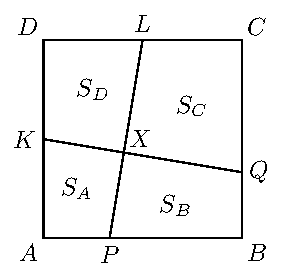
\includegraphics{obrazky/60D31}\\

Obr. 6
\end{center}

\\

\noindent \ul{21.5} [66-D-5-prvá časť] Ak označíme $X$ a $Y$ postupne stredy základní $RS$ a $TU$ všeobecného lichobežníka $RSTU$, tak na úsečke $XY$ leží priesečník $P$ uhlopriečok $RT$ a $SU$, a to tak, že $|PX| : |PY | = |RS| : |TU|$. Na priamke $XY$ leží tiež priesečník $Q$ predĺžených ramien $RU$ a $ST$, a to tak, že $|QX| : |QY | = |RS| : |TU|$ (obr. 9). Dokážte.


\\

\noindent \ul{21.6} [66-D-5] V danom trojuholníku ABC zvoľme vnútri strany $AC$ body $K$, $M$ a vnútri strany $BC$ body $L$, $N$ tak, že
$$|AK| = |KM| = |MC|, |BL| = |LN| = |NC|.$$
Ďalej označme $E$ priesečník uhlopriečok lichobežníka $ABLK$, $F$ priesečník uhlopriečok lichobežníka $KLNM$ a $G$ priesečník uhlopriečok lichobežníka $ABNM$. Dokážte, že body $E$, $F$ a $G$ ležia na ťažnici trojuholníka $ABC$ z vrcholu $C$ a určte pomer $|GF| : |EF|$.


\\

\section*{Seminár 22}

\noindent \ul{22.1} [66-K-3] Dokážte, že obdĺžnik s rozmermi $32 \times 120$ sa dá zakryť siedmimi zhodnými štvorcami so stranou 30.


\\

\noindent \ul{22.2} [60-S-2]  Daný je štvorec so stranou dĺžky 6\,cm. Nájdite množinu stredov všetkých priečok štvorca, ktoré ho delia na dva štvoruholníky, z ktorých jeden má obsah 12\,cm$^2$. (Priečka štvorca je úsečka, ktorej krajné body ležia na stranách štvorca.)


\\

\section*{Seminár 23}

\section*{Seminár 24}

\noindent \ul{24.1} [66-K-2]
Štvorcovú tabuľku $6\times 6$ zaplníme všetkými celými číslami od 1 do 36.

a) Uveďte príklad takého zaplnenia tabuľky, že súčet každých dvoch čísel v rovnakom riadku či v rovnakom stĺpci je väčší ako 11.

b) Dokážte, že pri ľubovoľnom zaplnení tabuľky sa v niektorom riadku alebo stĺpci nájdu dve čísla, ktorých súčet neprevyšuje 12.


\\

\noindent \ul{24.2} [62-D-1-N1]
Kobylka skáče po úsečke dĺžky 10\,cm a to skokmi o 1\,cm alebo o 2\,cm (vždy rovnakým smerom). Koľkými spôsobmi sa môže dostať z jedného krajného bodu úsečky do druhého?


\\

\noindent \ul{24.3} [62-D-2-N2, upravené] Škriatok sa pohybuje v tabuľke $10 \times 15$ skokmi o jedno políčko nahor alebo o jedno políčko doprava. Koľkými rôznymi cestami sa môže dostať z ľavého dolného do pravého horného políčka?\


\\

\noindent \ul{24.4} [64-K-2] V jednom políčku šachovnice $8 \times 8$ je napísané ”$-$“ a v ostatných políčkach ”$+$“. V jednom kroku môžeme zmeniť na opačné súčasne všechny štyri znamienka v ktoromkoľvek štvorci $2 \times 2$ na šachovnici. Rozhodnite, či po určitom počte krokov môže byť na šachovnici oboch znamienok rovnaký počet.


\\

\noindent \ul{24.5} [64-D-3-N3] Simona a Lenka hrajú hru. Pre dané celé číslo $k$ také, že $0 \leq k \leq 9$, vyberie Simona $k$ políčok šachovnice $3 \times 3$ a na každé z nich napíše číslo 1, na ostatné políčka napíše číslo 0. Lenka potom šachovnicu nejakým spôsobom pokryje tromi triminovými kockami, t. j. kockami tvaru $3\times1$, a čísla pod ich políčkami vynásobí. Ak je počet kociek so súčinom 0 nepárny, vyhráva Simona, v ostatných prípadoch vyhráva Lenka. Určte, v koľkých percentách prípadov (vzhľadom na hodnotu $k$) má vyhrávajúcu stratégiu Simona.


\\

\noindent \ul{24.6} [61-D-6-N1] Na hracej ploche $m\times n$ tvorenej bielymi štvorcovými políčkami sa Monika a Tamara striedajú v ťahoch jednou figúrkou pri nasledujúcej hre. Najskôr Monika položí figúrku na ľubovoľné políčko a toto políčko zafarbí namodro. Ďalej vždy hráčka, ktorá je na ťahu, urobí s figúrkou skok na políčko, ktoré je doposiaľ biele a zafarbí toto políčko namodro. Pritom pod skokom rozumieme ťah šachovou vežou, t. j. presuny figúrky v smere riadkov alebo v smere stĺpcov hracej dosky (o ľubovoľný počet políčok). Hráčka, ktorá je na rade a už nemôže urobiť ťah, prehráva. Rozhodnite, ktoré z hráčok môže hrať tak, že vyhrá nezávisle na ťahoch druhej hráčky?


\\

\noindent \ul{24.7} [62-D-1]
Štvorcová tabuľka je rozdelená na $16\times16$ políčok. Kobylka sa po nej pohybuje dvoma smermi: vpravo alebo dole, pričom strieda skoky o dve a o tri políčka (t. j. žiadne dva po sebe idúce skoky nie sú rovnako dlhé). Začína skokom dĺžky dva z ľavého horného políčka. Koľkými rôznymi cestami sa môže kobylka dostať na pravé dolné políčko? (Pod cestou máme na mysli postupnosť políčok, na ktoré kobylka doskočí.)


\\

\noindent \ul{24.8} [61-D-6]
Na hracej ploche $n \times n$ tvorenej bielymi štvorcovými políčkami sa Monika a Tamara striedajú v ťahoch jednou figúrkou pri nasledujúcej hre. Najskôr Monika položí figúrku na ľubovoľné políčko a toto políčko zafarbí namodro. Ďalej vždy hráčka, ktorá je na ťahu, urobí s figúrkou skok na políčko, ktoré je doposiaľ biele, a toto políčko zafarbí namodro. Pritom pod skokom rozumieme bežný ťah šachovým jazdcom, t. j. presun figúrky o dve políčka zvislo alebo vodorovne a súčasne o jedno políčko v druhom smere. Hráčka, ktorá je na rade a už nemôže urobiť ťah, prehráva. Postupne pre $n = 4, 5, 6$ rozhodnite, ktorá z hráčok môže hrať tak, že vyhrá nezávisle na ťahoch druhej hráčky.


\\

\section*{Seminár 25}

\noindent \ul{25.1} [61-D-6-N2] Na tabuli sú napísané všechny prvočísla menšie ako 100. Gitka a Terka sa striedajú v ťahoch pri nasledujúcej hre. Najprv Gitka zmaže jedno z prvočísel. Ďalej vždy hráčka, ktorá je na ťahu, zmaže jedno z prvočísel, ktoré má s predchádzajúcim zmazaným prvočíslom jednu zhodnú číslicu (tak po prvočísle 3 je možné zmazať trebárs 13 alebo 37). Hráčka, ktorá je na ťahu a nemôže už žiadne prvočíslo zmazať, prehráva. Ktorá z oboch hráčok môže hrať tak, že vyhrá nezávisle od ťahov súperky?


\\

\noindent \ul{25.2} [61-K-4] Na tabuli je napísaných prvých $n$ celých kladných čísel. Marína a Tamara sa striedajú v ťahoch pri nasledujúcej hre. Najskôr Marína zotrie jedno z čísel na tabuli. Ďalej vždy hráčka, ktorá je na ťahu, zotrie jedno z čísel, ktoré sa od predchádzajúceho zotretého čísla ani nelíši o 1, ani s ním nie je súdeliteľné. Hráčka, ktorá je na ťahu a nemôže už žiadne číslo zotrieť, prehrá. Pre $n = 6$ a pre $n = 12$ rozhodnite, ktorá z hráčok môže hrať tak, že vyhrá nezávisle na ťahoch druhej hráčky.


\\

\noindent \ul{25.3} [61-D-6-N3] Dve hráčky majú k dispozícii pre hru, ktorú opíšeme, neobmedzený počet dvadsaťcentových mincí a stôl s kruhovou doskou s priemerom 1\,m. Hra prebieha tak, že sa hráčky pravidelne striedajú v ťahoch. Najprv prvá hráčka položí jednu mincu kamkoľvek na prázdny stôl. Ďalej vždy hráčka, ktorá je na ťahu, položí na voľnú časť stola ďalšiu mincu (tak, aby nepresahovala okraj stola a aby sa skôr položených mincí nanajvýš dotýkala). Ktorá z oboch hráčok môže hrať tak, že vyhrá nezávisle od ťahov súperky?


\\

\noindent \ul{25.4} V skupine $n$ ľudí ($n \geq 4$) sa niektorí poznajú. Vzťah \uv{poznať sa} je vzájomný: ak osoba $A$ pozná osobu $B$, tak aj $B$ pozná $A$ a nazývame ich dvojicou známych.

a) Dokážte, že ak medzi každými štyrmi osobami sú aspoň štyri dvojice známych, tak každé dve osoby, ktoré sa nepoznajú, majú spoločného známeho.

b) Zistite, pre ktoré $n \geq 4$ existuje skupina osôb, v ktorej sú medzi každými štyrmi osobami aspoň tri dvojice známych a súčasne sa niektoré dve osoby ani nepoznajú, ani nemajú spoločného známeho.

c) Rozhodnite, či v skupine šiestich osôb môžu byť v každej štvorici práve tri dvojice známych a práve tri dvojice neznámych.


\\

\section*{Seminár 26}

\section*{Seminár 27}

\section*{Seminár 28}

\section*{Seminár 29}

\section*{Seminár 30}

\noindent \ul{30.1} [57-D-5] \ToDo Určte všechny dvojice $a, b$ reálnych čísel, pre ktoré má každá z
kvadratických rovníc
$$ax^2 + 2bx + 1 = 0, \ \ \ \ bx^2 + 2ax + 1 = 0$$
dva rôzne reálne korene, pričom práve jeden z nich je spoločný obom rovniciam.


\\

\noindent \ul{30.2} [57-S-5] \ToDo
Určte všechny dvojice $(a, b)$ reálnych čísel, pro které mají rovnice
$$x^2 + (3a + b)x + 4a = 0, \ \ \ \  x^2 + (3b + a)x + 4b = 0$$
společný reálny kořen.


\\

\noindent \ul{30.4}[59-D-6] Reálne čísla $a$, $b$ majú túto vlastnosť: rovnica $x^2 -ax+b-1 = 0$ má v množine reálnych čísel dva rôzne korene, ktorých rozdiel je kladným koreňom rovnice $x^2 - ax + b + 1 = 0$.

a) Dokážte nerovnosť $b > 3$.

b) Pomocou $b$ vyjadrite korene oboch rovníc.


\\

\noindent \ul{30.5}[59-S-1] Určte všechny hodnoty reálnych parametrov $p, q$, pre ktoré má každá z rovníc
$$x(x - p) = 3 + q, \ \ \ \ x(x + p) = 3 - q$$
v obore reálnych čísel dva rôzne korene, ktorých aritmetický priemer je jedným z koreňov
zvyšnej rovnice.


\\

\noindent \ul{30.6} [62-K-1] Pre ľubovoľné reálne čísla $k\neq \pm 1$, $p \neq 0$ a $q$ dokážte tvrdenie: Rovnica
$$x^2+ px + q = 0$$
má v obore reálnych čísel dva korene, z ktorých jeden je $k$-násobkom druhého, práve vtedy, keď platí $kp^2 = (k + 1)^2 q$.


\\

\noindent \ul{30.7} [64-K-4]  Na tabuli je zoznam čísel $1, 2, 3, 4, 5, 6$ a \uv{rovnica}
$$\frac{\fbox{$\phantom{7}$}}{\fbox{$\phantom{7}$}}x^2+\frac{\fbox{$\phantom{7}$}}{\fbox{$\phantom{7}$}}x + \frac{\fbox{$\phantom{7}$}}{\fbox{$\phantom{7}$}}= 0.$$
Marek s Tomášom hrajú nasledujúcu hru. Najskôr Marek vyberie ľubovoľné číslo zo zoznamu, napíše ho do jedného z prázdnych políčok v \uv{rovnici} a číslo zo zoznamu zotrie. Potom Tomáš vyberie niektoré zo zvyšných čísel, napíše ho do iného prázdneho políčka a v zozname ho zotrie. Nato Marek urobí to isté a nakoniec Tomáš doplní tri zvyšné čísla na tri zvyšné voľné políčka v \uv{rovnici}. Marek vyhrá, ak vzniknutá kvadratická rovnica s racionálnymi koeficientmi bude mať dva rôzne reálne korene, inak vyhrá Tomáš. Rozhodnite, ktorý z hráčov môže vyhrať nezávisle na postupe druhého
hráča.


\\

\section*{Seminár 31}

\section*{Seminár 32}

\section*{Seminár 33}

\section*{Seminár 34}

\section*{Seminár 4: Nerovnosti I}

\noindent \ul{4.1} [62-D-2-D4, resp. 55-C-II-2] Ak reálne čísla $a, b, c, d$ spĺňajú rovnosti $$a^2+ b^2= b^2+ c^2= c^2+ d^2= 1,$$
platí nerovnost
$$ab + ac + ad + bc + bd + cd \leq 3.$$
Dokážte a zistite, kedy za daných podmienok nastane rovnosť.


\\

\noindent \ul{4.2} [61-K-1]
Pre všechny reálne čísla $x, y, z$ také, že $x < y < z$, dokážte nerovnosť $$x^2 - y^2
+ z^2> (x - y + z)^2.$$


\\

\section*{Seminár 7: Deliteľnosť}

\noindent \ul{7.1} [60-D-2-N1] Ukážte, že každé prvočíslo väčšie ako 3 sa dá napísať v tvare $6k + 1$ alebo $6k - 1$ pre vhodné prirodzené číslo $k$.


\\

\noindent \ul{7.2} [60-D-2-N2] Nech $x + 5y$ dáva zvyšok 1 po delení 7. Aký zvyšok po delení 7 dáva číslo $3x + 15y$? A číslo $4x + 13y$?


\\

\noindent \ul{7.3} [60-S-3] Nech $x, y$ sú také kladné celé čísla, že obe čísla $3x + 5y$ a $5x + 2y$ sú deliteľné číslom 60. Zdôvodnite, prečo číslo 60 delí aj súčet $2x + 3y$.


\\

\noindent \ul{7.4} [60-D-2-D1] Dokážte, že ak pre celé čísla $a, b, c$ platí $7 | a - 3b + 5c$, tak platí aj $7 | 4a + 2b - c$. Zistite, či platí opačná implikácia.


\\

\noindent \ul{7.5} [60-D-2-D2] Dokážte, že ku každému celému číslu $x$ existuje celé číslo $y$ také, že $19x+3y$ je deliteľné 50.


\\

\noindent \ul{7.6} [63-D-5] Dokažte, že pro každé liché přirozené číslo $n$ je
součet $n^4 + 2n^2 + 2 013$ dělitelný číslem 96.

\\

\noindent \ul{7.7} [62-D-2-N2, resp. 50-S-3] Pre ktoré dvojciferné čísla $n$ je číslo $n^3 - n$ deliteľné číslom sto?


\\

\section*{Seminár 8: Najmenší spoločný násobok a najväčší spoločný deliteľ}

\noindent \ul{8.1} [61-D-3-N3 resp. 60-D-5-D1 resp. 50-C-S-1] Nájdite všechny trojice $a, b, c$ prirodzených čísel, pre ktoré súčasne platí $(ab, c) = 2^8$, $(bc, a) = 2^9$ a $(ca, b) = 2^{11}$. \\
\\
\ul{8.2} [64-D-5-N2] Rozdiel dvoch prirodzených čísel je 5 a ich najväčší spoločný deliteľ je 6-krát menší ako ich najmenší spoločný násobok. Určte obe také dvojice čísel.\\
\\
\ul{8.3} [62-S-1]
Určte všechny dvojice $a, b$ celých kladných čísel, pro které platí
$$a \cdot [a, b] = 4 \cdot (a, b),$$
pričom symbol $[a, b]$ označuje najmenší spoločný násobok a $(a, b)$ najväčší spoločný deliteľ celých kladných čísel $a, b$.


\\

\noindent \ul{8.4} [60-D-5-D2 resp. 50-C-I-3] Nájdite všechny dvojice prirodzených čísel $a, b$, pro které platí $[a, b] + (a, b) = 63$.\\
\\
\ul{8.5} [60-D-5-N3] Ukážte, že výraz $[a, 15]/a$, kde $a$ je prirodzené číslo, môže nadobúdať len štyri rôzne hodnoty, ktoré sú všechny celočíselné. Koľko rôznych celočíselných hodnôt môže nadobudnúť výraz $[120, b]/2b$? [Výraz $[60, b]/2b$ môže nadobudnúť celočíselné hodnoty 1, 2, 3, 5, 6, 10, 15, 30, okrem toho nadobúda hodnoty 1/2, 3/2, 5/2, 15/2.]

\\

\section*{Seminár 9: Ciferné zápisy}

\noindent \ul{9.1}  59-D-6 Nájdite všechny prirodzené čísla, ktoré nie sú deliteľné desiatimi a ktoré vo svojom dekadickom zápise majú niekde vedľa seba dve nuly, po ktorých vyškrtnutí sa pôvodné číslo 89-krát zmenší.


\\

\noindent \ul{9.2} [59-D-6-D1, resp. 56-K-4] Určte najväčšie dvojciferné číslo $k$ s nasledujúcou vlastnosťou: existuje prirodzené číslo $N$, z ktorého po škrtnutí prvej číslice zľava dostaneme číslo $k$-krát menšie. (Po škrtnutí číslice môže zápis čísla začínať jednou či niekoľkými nulami.) K určenému číslu $k$ potom nájdite najmenšie vyhovujúce číslo $N$.


\\

\noindent \ul{9.3} [58-D-3-N3, resp. 52-C-I-5] K prirodzenému číslu $m$ zapísanému rovnakými ciframi sme pripočítali štvorciferné prirodzené číslo $n$. Získali sme štvorciferné číslo s opačným poradím cifier, ako má číslo $n$. Určte všechny také dvojice čísel $m$ a $n$.


\\

\section*{Seminár 13: Kružnice}

\noindent \ul{13.1} [65-S-3] V kružnici so stredom $S$ zostrojíme priemer $AB$ a ľubovoľnú naň kolmú tetivu $CD$. Zdôvodnite, prečo je obvod trojuholníka $ACD$ menší ako dvojnásobok obvodu trojuholníka $SBC$.


\\

\noindent \ul{13.2} [59-S-2] Kružnice $k(S; 6\,\text{cm})$ a $l(O; 4\,\text{cm})$ majú vnútorný dotyk v bode $B$. Určte dĺžky strán trojuholníka $ABC$, pričom bod $A$ je priesečník priamky $OB$ s kružnicou $k$ a bod $C$ je priesečník kružnice $k$ s dotyčnicou z bodu $A$ ku kružnici $l$.


\\

